%!TEX root = ../paper.tex
In this section we present the results of the two estimators on dataset \ferdosiTwo, \baakmanTwo, \ferdosiThree, \baakmanThree, \ie the datasets that contain more than one Gaussian.

The plots in \cref{fig:4:resuts:multiSphere} suggest some differences in how the two estimators handle the different components of the dataset, therefore \cref{tab:4:results:multisphere:componentmse} presents the mean square error of the different components of the datasets that contain multiple Gaussians. 

\begin{table*}
	\centering
	%!TEX root = ../paper.tex

\begin{tabular}{@{}ccl*{2}{S[scientific-notation=true,round-mode=places,round-precision=3]}}
\toprule
~				&~					&~ 				& \multicolumn{2}{c}{Estimator}\\ \cmidrule{4-5}
Set 			&~					& Component		& {\mbe} 				& {\sambe}\\
\midrule
% Ferdosi 2
\hline
\ferdosiTwo 	&\legendDot{blue}	& Gaussian 1	& 1.560536961708337e-07 & 2.993178935719230e-07\\
~ 				&\legendDot{green}	& Gaussian 2	& 2.285260303722557e-09 & 8.344636264610111e-10\\
				&\legendDot{red}	& Noise 		& 2.021379766292543e-11 & 2.363141221512672e-11\\
% Ferdosi 3
\hline
\ferdosiThree	&\legendDot{blue}	& Gaussian 1	& 0.0 & 0.0\\
~ 				&\legendDot{green}	& Gaussian 2	& 0.0 & 0.0\\
~ 				&\legendDot{red}	& Gaussian 3	& 0.0 & 0.0\\
~ 				&\legendDot{orange}	& Gaussian 4	& 0.0 & 0.0\\
% Baakman 2
\hline
\baakmanTwo		&\legendDot{blue}	& Gaussian 1	& 0.0 & 0.0\\
~ 				&\legendDot{green}	& Gaussian 2	& 0.0 & 0.0\\
% Baakman 3
\hline
\baakmanThree	&\legendDot{blue}	& Gaussian 1 	& 0.0 & 0.0 \\
~ 				&\legendDot{green}	& Gaussian 2 	& 0.0 & 0.0 \\
~ 				&\legendDot{red}	& Gaussian 3 	& 0.0 & 0.0 \\
~ 				&\legendDot{orange}	& Gaussian 4 	& 0.0 & 0.0 \\
\bottomrule
\end{tabular}
	\caption{The mean squared error of the known densities and the densities estimated by the Modified Breiman Estimator (\mbe) and the shape-adaptive MBE (\sambe), respectively, for the different components of the datasets with multiple Gaussians.} 	
	\label{tab:4:results:multisphere:componentmse}
\end{table*}

% Ferdosi 2 & Baakman 2
	% MSE
	\Cref{tab:4:results:multisphere:componentmse} shows some difference in MSE between the different components of dataset \ferdosiTwo, and the elongated version of this dataset, \ie dataset \baakmanTwo: both estimators perform best on data points that were drawn from the uniform distribution, and worst on Gaussian 1, the Gaussian component with the smallest radius. Furthermore \sambe outperforms \mbe on the component named `Gaussian 2'.

	% Plots
	Comparing \cref{fig:4:results:mbe:ferdosi2,fig:4:results:mbe:baakman2,fig:4:results:sambe:ferdosi2,fig:4:simulated:datasets:sambe:baakman2} we find that on both datasets both estimators underestimate the density. Although the ranges of the densities estimated by \sambe are slightly higher than those estimated by the Modified Breiman Estimator the ranges do not differ as extremely as they did when a single non-spherical Gaussian with noise made up the dataset. 

% Ferdosi 3 & Baakman 3
	% MSE

	% Plots

	\todo[inline]{Report on \cref{fig:4:results:mbe:ferdosi3} and \cref{fig:4:results:mbe:baakman3}.}

% General
	\todo[inline]{General observation of multi sphere datasets.}


\begin{figure*}
	\centering
	%!TEX root = ../paper.tex

% Ferdosi 2, MBE
\begin{subfigure}{0.23\textwidth}
	\centering
	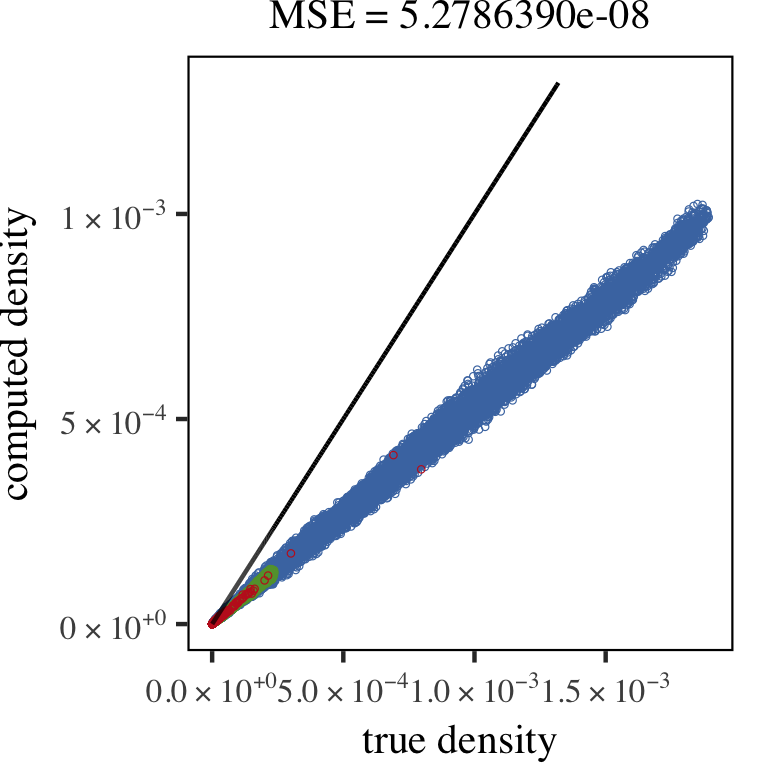
\includegraphics[keepaspectratio=true, width=\textwidth, height=0.23\textheight]{result/img/all/results_ferdosi_2_60000_mbe_silverman}
	\caption{Set \ferdosiTwo, \mbe}
	\label{fig:4:results:mbe:ferdosi2}
\end{subfigure}
% Baakman 2, MBE
\begin{subfigure}{0.23\textwidth}
	\centering
	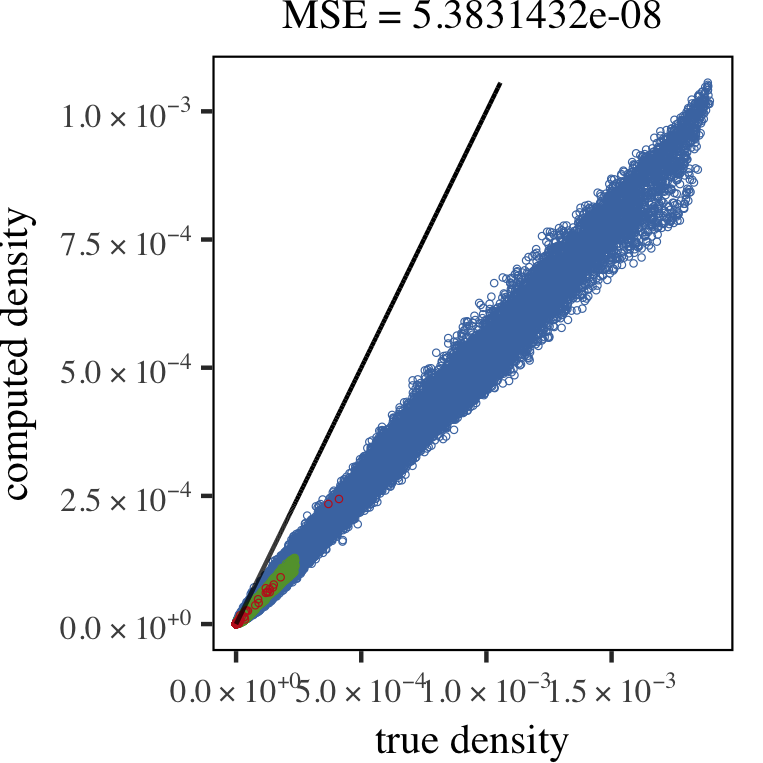
\includegraphics[keepaspectratio=true, width=\textwidth, height=0.23\textheight]{result/img/all/results_baakman_2_60000_mbe_silverman}
	\caption{Set \baakmanTwo, \mbe}
	\label{fig:4:results:mbe:baakman2}
\end{subfigure}
% Ferdosi 3, MBE
\begin{subfigure}{0.23\textwidth}
	\centering
	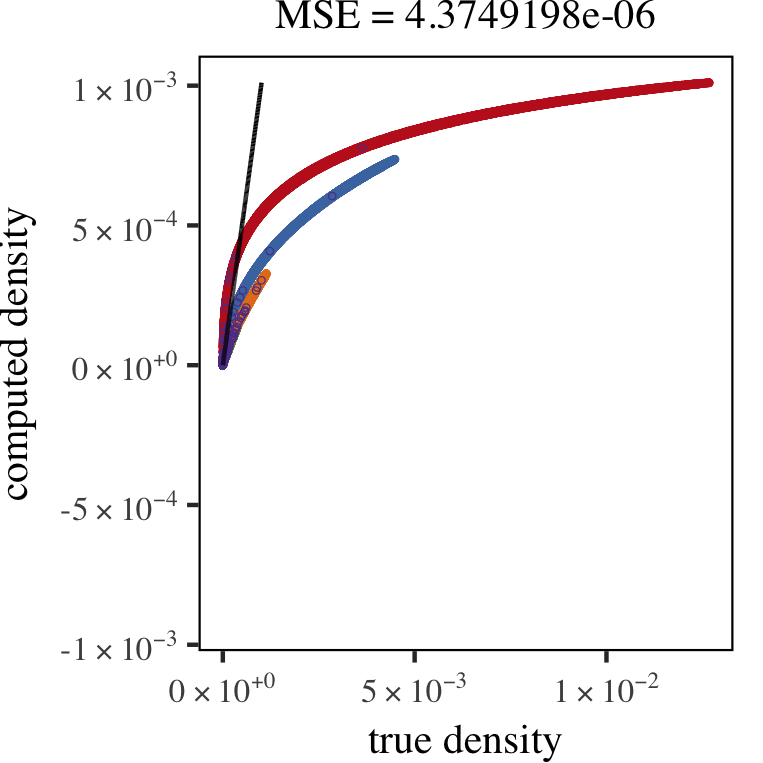
\includegraphics[keepaspectratio=true, width=\textwidth, height=0.23\textheight]{result/img/all/results_ferdosi_3_120000_mbe_silverman.png}
	\caption{Set \ferdosiThree, \mbe}
	\label{fig:4:results:mbe:ferdosi3}
\end{subfigure}
% Baakman 3, MBE
\begin{subfigure}{0.23\textwidth}
	\centering
	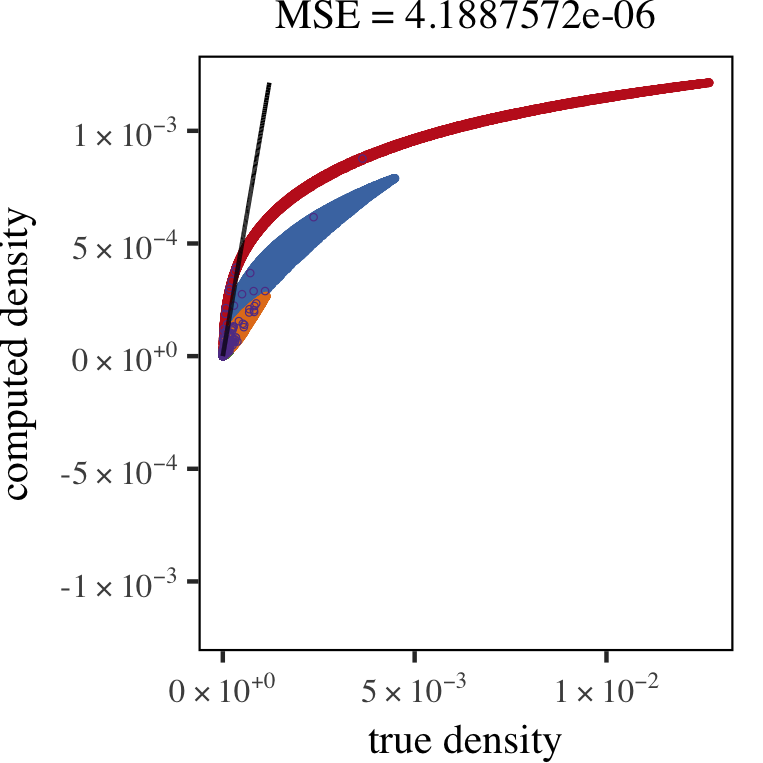
\includegraphics[keepaspectratio=true, width=\textwidth, height=0.23\textheight]{result/img/all/results_baakman_3_120000_mbe_silverman}
	\caption{Set \baakmanThree, \mbe}
	\label{fig:4:results:mbe:baakman3}
\end{subfigure}	
% Ferdosi 2, SAMBE
\begin{subfigure}{0.23\textwidth}
	\centering
	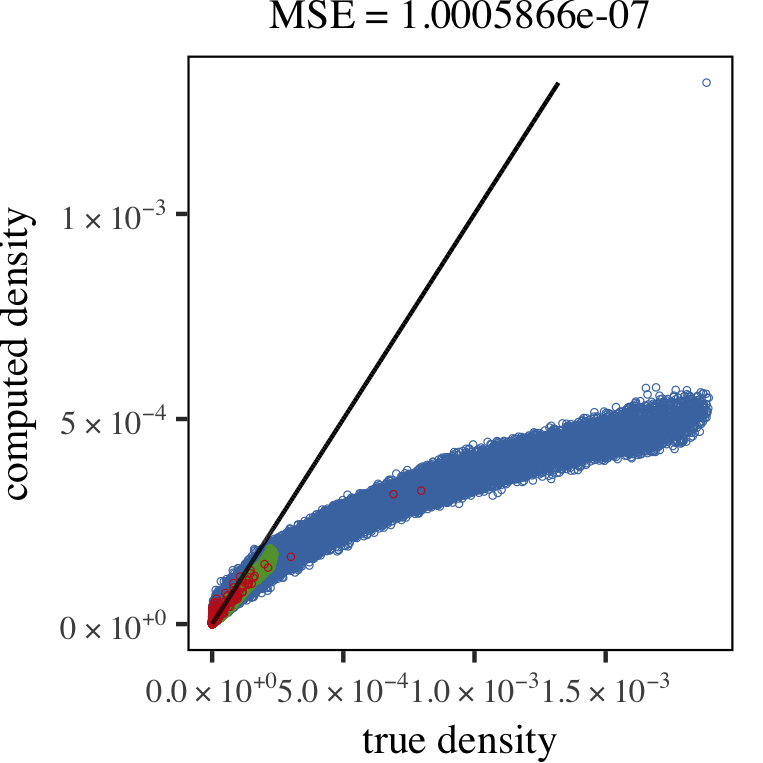
\includegraphics[keepaspectratio=true, width=\textwidth, height=0.23\textheight]{result/img/all/results_ferdosi_2_60000_sambe_silverman}
	\caption{Set \ferdosiTwo, \sambe}
	\label{fig:4:results:sambe:ferdosi2}
\end{subfigure}
% Baakman 2, SAMBE
\begin{subfigure}{0.23\textwidth}
	\centering
	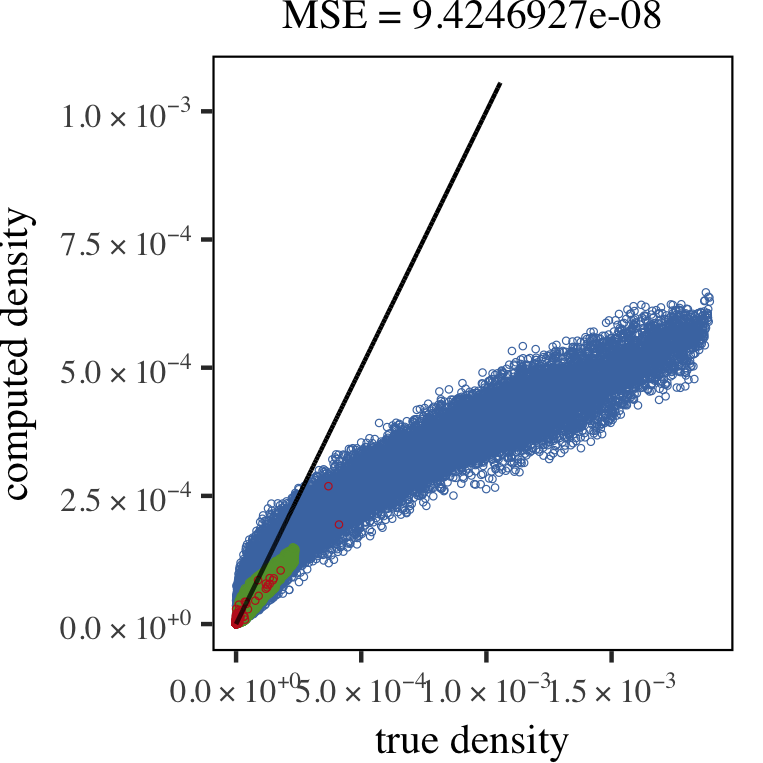
\includegraphics[keepaspectratio=true, width=\textwidth, height=0.23\textheight]{result/img/all/results_baakman_2_60000_sambe_silverman}
	\caption{Set \baakmanTwo, \sambe}
	\label{fig:4:simulated:datasets:sambe:baakman2}
\end{subfigure}
% Ferdosi 3, SAMBE
\begin{subfigure}{0.23\textwidth}
	\centering
	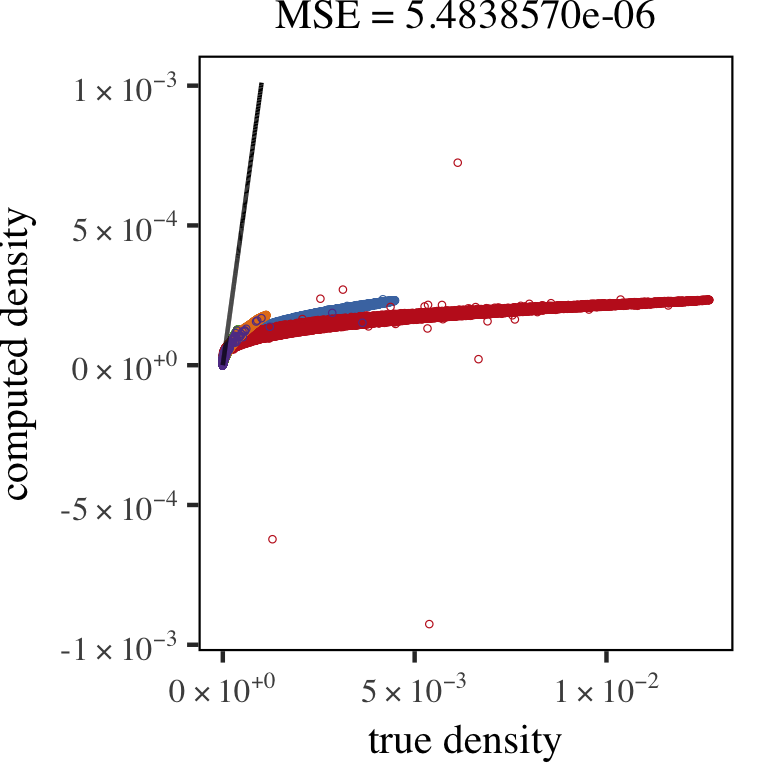
\includegraphics[keepaspectratio=true, width=\textwidth, height=0.23\textheight]{result/img/all/results_ferdosi_3_120000_sambe_silverman}
	\caption{Set \ferdosiThree, \sambe}
	\label{fig:4:simulated:datasets:sambe:ferdosi3}
\end{subfigure}
% Baakman 3, SAMBE
\begin{subfigure}{0.23\textwidth}
	\centering
	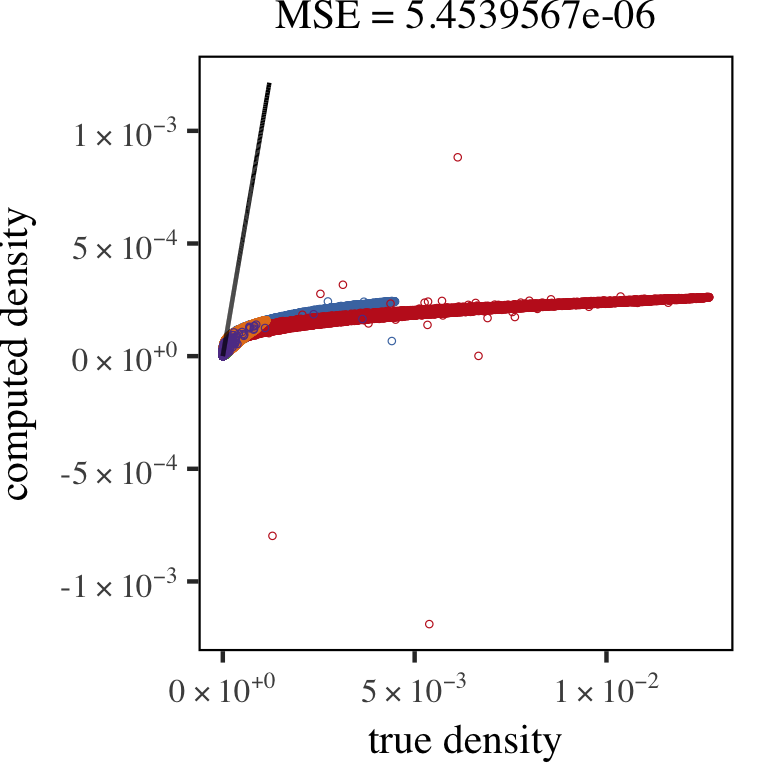
\includegraphics[keepaspectratio=true, width=\textwidth, height=0.23\textheight]{result/img/all/results_baakman_3_120000_sambe_silverman}
	\caption{Set \baakmanThree, \sambe}
	\label{fig:4:results:sambe:baakman3}
\end{subfigure}	
	\caption{Comparative plots for dataset \ferdosiTwoNum, \ferdosiThreeNum, \baakmanTwoNum, and \baakmanThreeNum.}
	\label{fig:4:resuts:multiSphere}
\end{figure*}